\section{Paraphrasing Chunks}

Initially, we hypothesized that smaller chunks of text would lead to better paraphrases, 
since smaller chunks are easer to process and control in terms of topic,
suggesting that the separation of text into smaller chunks would be beneficial for the paraphrasing process.
We therefore designed an ablation study to test this hypothesis.
We computed several paraphrasing measurements for the same input texts averaged over the number of chunks.
As visualized in \autoref{fig:abl_chunks_T5_Google_PAWS} and \autoref{fig:abl_chunks_BulletPoint},
the syntactic scores of naive paraphrasers (here: \ac{t5} model) increase with the number of chunks,
while the semantic scores remain stable.
This leads to a decreasing Gohsen Delta score, which is the difference between the semantic and syntactic scores.
In contrast, the non-naive paraphrasers (here: BulletPoint model) do not show any significant change in the paraphrasing scores with the number of chunks.
This suggests that the naive paraphrasers are more sensitive to the number of chunks, 
while the non-naive model is not affected by it.
Since a large Gohsen Delta score indicates a good paraphrase,
the results suggest that the naive paraphrasers perform better with fewer chunks, 
while the non-naive paraphrasers are more robust to the number of chunks.
This finding indicates that more chunks allow for better syntactic control, which is not necessarily beneficial for the quality of the paraphrase.
As we are interested in syntactically diverse paraphrases,
we will not use chunks for the paraphrasing process but rather stick to text-to-text paraphrases.
 
\begin{figure}[htbp]
    \centering
    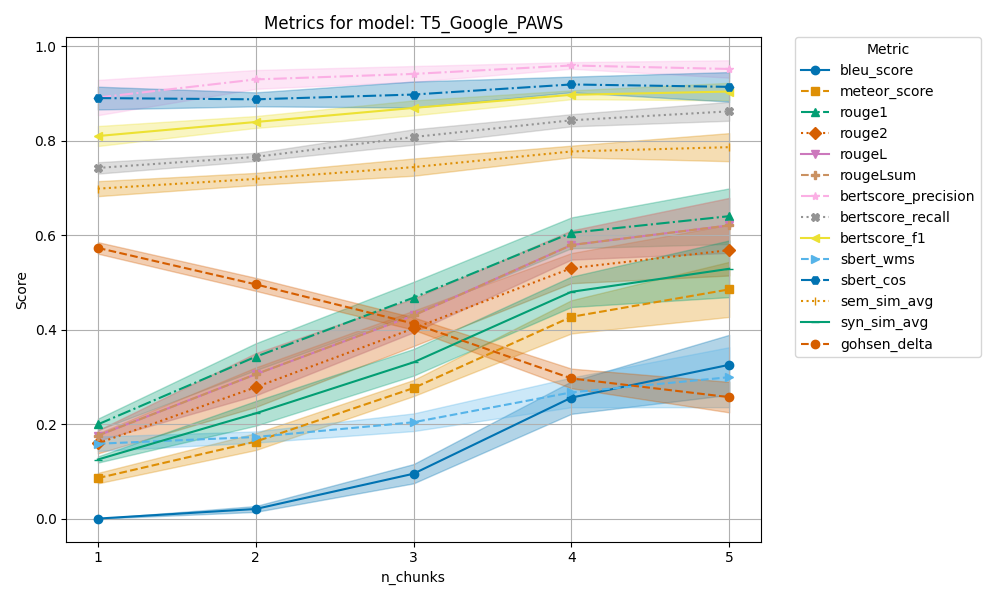
\includegraphics[width=\textwidth]{images/paraphrasing/experiments/T5_Google_PAWS_metrics_plot.png}
    \caption{Average score over different prompts (standard deviation shaded) for different paraphrasing scores for the \ac{t5} model.
    The syntactic scores rise with the number of chunks, while the semantic scores is stable.
    Consequently, the Gohsen Delta score is decreasing with the number of chunks.}
    \label{fig:abl_chunks_T5_Google_PAWS}
\end{figure}

\begin{figure}[htbp]
    \centering
    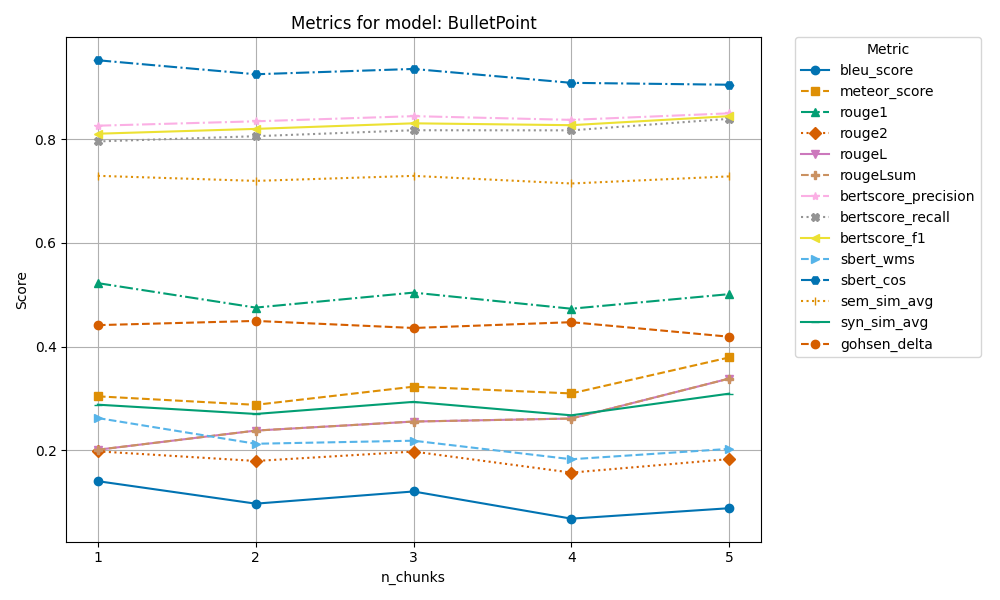
\includegraphics[width=\textwidth]{images/paraphrasing/experiments/BulletPoint_metrics_plot.png}
    \caption{Different paraphrasing scores for the BulletPoint model. 
    This model is not affected by the number of chunks.}
    \label{fig:abl_chunks_BulletPoint}
\end{figure}